
\newcommand{\thegivenstuff}[0]{
Given Object set: $O = \{A, B, C, D, E\}$ \\ \newline
Given Matrix: 
\[
\begin{array}{c|ccccc}
  & A & B & C & D & E \\
\hline
A & 0 & 6 & 8 & 12 & 8 \\
B &   & 0 & 2 & 14 & 4 \\ 
C &   &   & 0 & 12 & 4 \\ 
D &   &   &   & 0 & 16 \\
E &   &   &   &   & 0
\end{array}
\]
}

\tikzset{
    punkt/.style={circle, fill, inner sep=1.5pt}
}


\newcommand{\stepone}[0]{1. Find the two clusters $i$ and $j$ $i \neq j$ with the smallest distance $d_{ij}$.}
\newcommand{\steptwo}[0]{2. Create a new cluster $u$ that joins clusters $i$ and $j$.}
\newcommand{\stepthree}[0]{3. Define the height (i.e. distance from leaves) of $u$ to be $l_{ij} := d_{ij} /2$}
\newcommand{\stepfour}[0]{4. Compute the distance $d_{ku}$ of $u$ to any other cluster $k \notin \{i, j\}$ in one of the ways described below.}
\newcommand{\stepfive}[0]{5. Replace clusters $i$ and $j$ by the new cluster $u$.}

\subsection*{Agglomerative Clustering}

\subsubsection*{General strategy}

While there is more than one cluster left, do:
\begin{itemize}
    \item[] \stepone
    \item[] \steptwo
    \item[] \stepthree
    \item[] \stepfour
    \item[] \stepfive
\end{itemize}

\subsubsection{Single linkage clustering}
\thegivenstuff
\subsubsection*{First iteration}
\paragraph{\stepone}
\[
d_{BC} = 2
\]
\paragraph*{\steptwo}
New cluster: (BC) 
\paragraph*{\stepthree}
\[l_{BC} := 2 /2 = 1\] \\
\begin{center}
    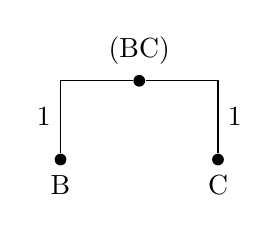
\begin{tikzpicture}
        \path node[punkt, label=above:(BC)] (BC) at (0,0) {}
        node[punkt, label=below:B] (B) at (-1,-1) {} 
        node[punkt, label=below:C] (C) at (1,-1) {};
        \draw   (BC) -| node[near end, left] {1} (B);
        \draw   (BC) -| node[near end, right] {1} (C);
    \end{tikzpicture} 
\end{center}
\paragraph*{\stepfour}
\begin{align*}
    d_{A, (BC)} & = min(d_{A,B}, d_{(A,C)}) = min (6,8) = 6 \\
    d_{D, (BC)} & = min(d_{D,B}, d_{(D,C)}) = min (14,12) = 12 \\
    d_{E, (BC)} & = min(d_{E,B}, d_{(E,C)}) = min (4,4) = 4 
\end{align*}
\paragraph*{\stepfive}
\[
\begin{array}{c|ccccc}
  & A & (BC) & D & E \\
\hline
A & 0& 6 & 12& 8 \\
(BC) &  & 0 & 12 & 4 \\
D &  &   & 0 & 16 \\
E &  &   &   & 0
\end{array}
\]
\subsubsection*{Second interation}
\paragraph*{\stepone}
\[d_{(BC),E} = 4\]
\paragraph*{\steptwo}
New cluster: ((BC)E)
\paragraph*{\stepthree}
\[l_{(BC)E} := 4 /2 = 2\] \\
\begin{center}
    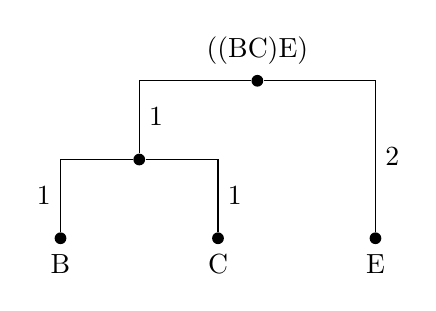
\begin{tikzpicture}
    \path node[punkt] (BC) at (0,0) {}
        node[punkt, label=below:B] (B) at (-1,-1) {}
        node[punkt, label=below:C] (C) at (1,-1) {}
        node[punkt, label=below:E] (E) at (3,-1) {}
        node[punkt, label=above:((BC)E)] (BCE) at (1.5,1) {};
       \draw   (BC) -| node[near end,left] {1} (B);
        \draw   (BC) -| node[near end,right] {1} (C);
        \draw   (BCE) -| node[near end,right] {2} (E);
        \draw   (BCE) -| node[near end,right] {1} (BC);
    \end{tikzpicture}
\end{center}
\paragraph*{\stepfour}
\begin{align*}
    d_{A, ((BC)E)} & = min(d_{A,BC}, d_{(A,E)}) = min (6,8) = 6 \\
    d_{D, ((BC)E)} & = min(d_{D,BC}, d_{(D,E)}) = min (12,16) = 12 
\end{align*}
\paragraph*{\stepfive}
\[
\begin{array}{c|ccccc}
  & A & ((BC)E) & D \\
\hline
A & 0& 6 & 12 \\
((BC)E) &  & 0 & 12  \\
D &  &   & 0
\end{array}
\]
\subsubsection*{Third iteration}
\paragraph*{\stepone}
\[d_{((BC)E) A} = 6\]
\paragraph*{\steptwo}
New cluster: (A((BC)E))
\paragraph*{\stepthree}
\[l_{((BC)E) A} := 6 /2 = 3\] \\
\begin{center}
    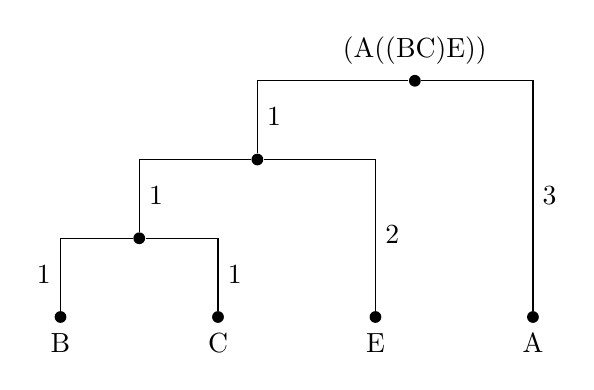
\begin{tikzpicture}
    \path node[punkt] (BC) at (0,0) {}
        node[punkt, label=below:B] (B) at (-1,-1) {}
        node[punkt, label=below:C] (C) at (1,-1) {}
        node[punkt, label=below:E] (E) at (3,-1) {}
         node[punkt, label=below:A] (A) at (5,-1) {}
        node[punkt, label=above:(A((BC)E))] (ABCE) at (3.5,2) {}
        node[punkt] (BCE) at (1.5,1) {};
       \draw   (BC) -| node[near end,left] {1} (B);
        \draw   (BC) -| node[near end,right] {1} (C);
        \draw   (BCE) -| node[near end,right] {2} (E);
        \draw   (BCE) -| node[near end,right] {1} (BC);
        \draw   (ABCE) -| node[near end,right] {1} (BCE);
        \draw   (ABCE) -| node[near end,right] {3} (A);
    \end{tikzpicture}
\end{center}
\paragraph*{\stepfour}
\begin{align*}
    d_{D, (A((BC)E))} & = min(d_{D,BCE}, d_{(D,A)}) = min (12,12) = 12 
\end{align*}
\paragraph*{\stepfive}
\[
\begin{array}{c|ccccc}
  &  (A((BC)E)) & D \\
\hline
(A((BC)E)) & 0 & 12  \\
D &    & 0
\end{array}
\]

\subsubsection*{Finale}
Join the last cluster. 
\[ l_{D, (A((BC)E))} = 12 / 2 = 6\]
\newcommand{\slcluster}[0]{ \begin{tikzpicture}
    \path node[punkt] (BC) at (0,0) {}
        node[punkt, label=below:B] (B) at (-1,-1) {}
        node[punkt, label=below:C] (C) at (1,-1) {}
        node[punkt, label=below:E] (E) at (3,-1) {}
         node[punkt, label=below:A] (A) at (5,-1) {}
         node[punkt, label=below:D] (D) at (7,-1) {}
        node[punkt] (ABCE) at (3.5,2) {}
         node[punkt] (ABCDE) at (5.5,5) {}
        node[punkt] (BCE) at (1.5,1) {};
       \draw   (BC) -| node[near end,left] {1} (B);
        \draw   (BC) -| node[near end,right] {1} (C);
        \draw   (BCE) -| node[near end,right] {2} (E);
        \draw   (BCE) -| node[near end,right] {1} (BC); 
        \draw   (ABCE) -| node[near end,right] {1} (BCE);
        \draw   (ABCE) -| node[near end,right] {3} (A);
         \draw   (ABCDE) -| node[near end,right] {6} (D);
         \draw   (ABCDE) -| node[near end,right] {3} (ABCE);
    \end{tikzpicture}}
\begin{center}
   \slcluster
\end{center}
\newpage

\newpage 
\subsubsection{Complete linkage clustering}
\thegivenstuff
\subsubsection*{First iteration}
\paragraph{\stepone}
\[
d_{BC} = 2
\]
\paragraph*{\steptwo}
New cluster: (BC) 
\paragraph*{\stepthree}
\[l_{BC} := 2 /2 = 1\] \\
\begin{center}
    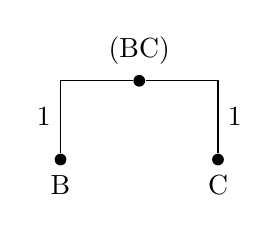
\begin{tikzpicture}
        \path node[punkt, label=above:(BC)] (BC) at (0,0) {}
        node[punkt, label=below:B] (B) at (-1,-1) {} 
        node[punkt, label=below:C] (C) at (1,-1) {};
        \draw   (BC) -| node[near end, left] {1} (B);
        \draw   (BC) -| node[near end, right] {1} (C);
    \end{tikzpicture} 
\end{center}
\paragraph*{\stepfour}
\begin{align*}
    d_{A, (BC)} & = max(d_{A,B}, d_{(A,C)}) = min (6,8) = 8 \\
    d_{D, (BC)} & = max(d_{D,B}, d_{(D,C)}) = min (14,12) = 14 \\
    d_{E, (BC)} & = max(d_{E,B}, d_{(E,C)}) = min (4,4) = 4 
\end{align*}
\paragraph*{\stepfive}
\[
\begin{array}{c|ccccc}
  & A & (BC) & D & E \\
\hline
A & 0& 8 & 12& 8 \\
(BC) &  & 0 & 14 & 4 \\
D &  &   & 0 & 12 \\
E &  &   &   & 0
\end{array}
\]
\subsubsection*{Second interation}
\paragraph*{\stepone}
\[d_{(BC),E} = 4\]
\paragraph*{\steptwo}
New cluster: ((BC)E)
\paragraph*{\stepthree}
\[l_{(BC)E} := 4 /2 = 2\] \\
\begin{center}
    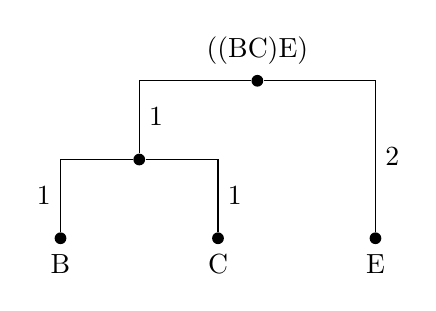
\begin{tikzpicture}
    \path node[punkt] (BC) at (0,0) {}
        node[punkt, label=below:B] (B) at (-1,-1) {}
        node[punkt, label=below:C] (C) at (1,-1) {}
        node[punkt, label=below:E] (E) at (3,-1) {}
        node[punkt, label=above:((BC)E)] (BCE) at (1.5,1) {};
       \draw   (BC) -| node[near end,left] {1} (B);
        \draw   (BC) -| node[near end,right] {1} (C);
        \draw   (BCE) -| node[near end,right] {2} (E);
        \draw   (BCE) -| node[near end,right] {1} (BC);
    \end{tikzpicture}
\end{center}
\paragraph*{\stepfour}
\begin{align*}
    d_{A, ((BC)E)} & = max(d_{A,BC}, d_{(A,E)}) = min (8,8) = 8 \\
    d_{D, ((BC)E)} & = max(d_{D,BC}, d_{(D,E)}) = min (14,12) = 14
\end{align*}
\paragraph*{\stepfive}
\[
\begin{array}{c|ccccc}
  & A & ((BC)E) & D \\
\hline
A & 0& 8 & 12 \\
((BC)E) &  & 0 & 14  \\
D &  &   & 0
\end{array}
\]
\subsubsection*{Third iteration}
\paragraph*{\stepone}
\[d_{((BC)E),A} = 8\]
\paragraph*{\steptwo}
New cluster: (A((BC)E))
\paragraph*{\stepthree}
\[l_{(A((BC)E)} := 8 /2 = 4\] \\
\begin{center}
    \begin{tikzpicture}
    \path node[punkt] (BC) at (0,0) {}
        node[punkt, label=below:B] (B) at (-1,-1) {}
        node[punkt, label=below:C] (C) at (1,-1) {}
        node[punkt, label=below:E] (E) at (3,-1) {}
         node[punkt, label=below:A] (A) at (5,-1) {}
        node[punkt, label=above:(A((BC)E))] (ABCE) at (3.5,3) {}
        node[punkt] (BCE) at (1.5,1) {};
       \draw   (BC) -| node[near end,left] {1} (B);
        \draw   (BC) -| node[near end,right] {1} (C);
        \draw   (BCE) -| node[near end,right] {2} (E);
        \draw   (BCE) -| node[near end,right] {1} (BC);
        \draw   (ABCE) -| node[near end,right] {2} (BCE);
        \draw   (ABCE) -| node[near end,right] {4} (A);
    \end{tikzpicture}
\end{center}
\paragraph*{\stepfour}
\begin{align*}
    d_{D, (A((BC)E))} & = max(d_{D,((BC)E)}, d_{(D,A)}) = min (14,12) = 14
\end{align*}
\paragraph*{\stepfive}
\[
\begin{array}{c|ccccc}
  &  (A((BC)E)) & D \\
\hline
(A((BC)E)) & 0 & 14  \\
D &    & 0
\end{array}
\]

\subsubsection*{Finale}
Join the last cluster. 
\[ l_{D, (A((BC)E))} = 14 / 2 = 7\]
\newcommand{\clcluster}[0]{    \begin{tikzpicture}
    \path node[punkt] (BC) at (0,0) {}
        node[punkt, label=below:B] (B) at (-1,-1) {}
        node[punkt, label=below:C] (C) at (1,-1) {}
        node[punkt, label=below:E] (E) at (3,-1) {}
         node[punkt, label=below:A] (A) at (5,-1) {}
         node[punkt, label=below:D] (D) at (7,-1) {}
        node[punkt] (ABCE) at (3.5,3) {}
         node[punkt] (ABCDE) at (5.5,6) {} 
        node[punkt] (BCE) at (1.5,1) {};
       \draw   (BC) -| node[near end,left] {1} (B);
        \draw   (BC) -| node[near end,right] {1} (C);
        \draw   (BCE) -| node[near end,right] {2} (E);
        \draw   (BCE) -| node[near end,right] {1} (BC);
        \draw   (ABCE) -| node[near end,right] {2} (BCE);
        \draw   (ABCE) -| node[near end,right] {4} (A);
         \draw   (ABCDE) -| node[near end,right] {7} (D);
         \draw   (ABCDE) -| node[near end,right] {3} (ABCE);
    \end{tikzpicture}}
\begin{center}
\clcluster
\end{center}
\newpage


\subsubsection{UPGMA}
\thegivenstuff
\subsubsection*{First iteration}
\paragraph{\stepone}
\[
d_{BC} = 2
\]
\paragraph*{\steptwo}
New cluster: (BC) 
\paragraph*{\stepthree}
\[l_{BC} := 2 /2 = 1\] \\
\begin{center}
    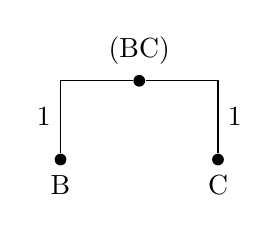
\begin{tikzpicture}
        \path node[punkt, label=above:(BC)] (BC) at (0,0) {}
        node[punkt, label=below:B] (B) at (-1,-1) {} 
        node[punkt, label=below:C] (C) at (1,-1) {};
        \draw   (BC) -| node[near end, left] {1} (B);
        \draw   (BC) -| node[near end, right] {1} (C);
    \end{tikzpicture} 
\end{center}
\paragraph*{\stepfour}
\begin{align*}
    d_{A, (BC)} & = \frac{n_{B} \cdot  d_{AB} + n_{C} \cdot  d_{AC}}{n_B + n_C}   = \frac{1 \cdot 6 + 1 \cdot 8}{1 + 1} = 7 \\
    d_{D, (BC)} & = \frac{n_{B} \cdot  d_{DB} + n_{C} \cdot  d_{DC}}{n_B + n_C}   = \frac{1 \cdot 14 + 1 \cdot 12}{1 + 1} = 13 \\
    d_{E, (BC)} & = \frac{n_{B} \cdot  d_{EB} + n_{C} \cdot  d_{EC}}{n_B + n_C}   = \frac{1 \cdot 4 + 1 \cdot 4}{1 + 1} = 4
\end{align*}
\paragraph*{\stepfive}
\[
\begin{array}{c|ccccc}
  & A & (BC) & D & E \\
\hline
A & 0& 7 & 12& 8 \\
(BC) &  & 0 & 13 & 4 \\
D &  &   & 0 & 12 \\
E &  &   &   & 0
\end{array}
\]
\subsubsection*{Second interation}
\paragraph*{\stepone}
\[d_{(BC),E} = 4\]
\paragraph*{\steptwo}
New cluster: ((BC)E)
\paragraph*{\stepthree}
\[l_{(BC)E} := 4 /2 = 2\] \\
\begin{center}
    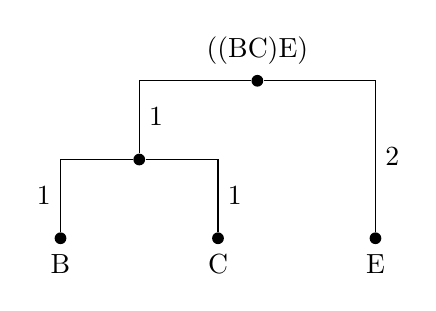
\begin{tikzpicture}
    \path node[punkt] (BC) at (0,0) {}
        node[punkt, label=below:B] (B) at (-1,-1) {}
        node[punkt, label=below:C] (C) at (1,-1) {}
        node[punkt, label=below:E] (E) at (3,-1) {}
        node[punkt, label=above:((BC)E)] (BCE) at (1.5,1) {};
       \draw   (BC) -| node[near end,left] {1} (B);
        \draw   (BC) -| node[near end,right] {1} (C);
        \draw   (BCE) -| node[near end,right] {2} (E);
        \draw   (BCE) -| node[near end,right] {1} (BC);
    \end{tikzpicture}
\end{center}
\paragraph*{\stepfour}
\begin{align*}
    d_{A, ((BC)E)} & = \frac{n_{(BC)} \cdot  d_{A(BC)} + n_{E} \cdot  d_{AE}}{n_{BC} + n_E}   = \frac{2 \cdot 7 + 1 \cdot 8}{2 + 1} = \frac{22}{3} \\
    d_{D, ((BC)E)} & = \frac{n_{(BC)} \cdot  d_{D(BC)} + n_{E} \cdot  d_{DE}}{n_{BC} + n_E}   = \frac{2 \cdot 13 + 1 \cdot 12}{2 + 1} = \frac{38}{3}
\end{align*}
\paragraph*{\stepfive}
\[
\begin{array}{c|ccccc}
  & A & ((BC)E) & D \\
\hline
A & 0& \frac{22}{3} & \frac{36}{3} \\
((BC)E) &  & 0 & \frac{38}{3}  \\
D &  &   & 0
\end{array}
\]
\subsubsection*{Third iteration}
\paragraph*{\stepone}
\[d_{((BC)E),A }= \frac{22}{3}\]
\paragraph*{\steptwo}
New cluster: (A((BC)E))
\paragraph*{\stepthree}
\[l_{BC} := \frac{22}{3} /2 = \frac{11}{3}\] \\
\begin{center}
    \begin{tikzpicture}
    \path node[punkt] (BC) at (0,0) {}
        node[punkt, label=below:B] (B) at (-1,-1) {}
        node[punkt, label=below:C] (C) at (1,-1) {}
        node[punkt, label=below:E] (E) at (3,-1) {}
         node[punkt, label=below:A] (A) at (5,-1) {}
        node[punkt, label=above:(A((BC)E))] (ABCE) at (3.5,2.6) {}
        node[punkt] (BCE) at (1.5,1) {};
       \draw   (BC) -| node[near end,left] {1} (B);
        \draw   (BC) -| node[near end,right] {1} (C);
        \draw   (BCE) -| node[near end,right] {2} (E);
        \draw   (BCE) -| node[near end,right] {1} (BC);
        \draw   (ABCE) -| node[near end,right] {$\frac{5}{3}$} (BCE);
        \draw   (ABCE) -| node[near end,right] {$\frac{11}{3}$} (A);
    \end{tikzpicture}
\end{center}
\paragraph*{\stepfour}
\begin{align*}
    d_{D, (A((BC)E))} & = \frac{n_{((BC)E)} \cdot  d_{D((BC)E)} + n_{A} \cdot  d_{DA}}{n_{((BC)E)} + n_A}   = \frac{3 \cdot \frac{38}{3} + 1 \cdot 12}{ 3 + 1} = \frac{50}{4} = \frac{25}{2} = \frac{37,5}{3}
\end{align*}
\paragraph*{\stepfive}
\[
\begin{array}{c|ccccc}
  &  (A((BC)E)) & D \\
\hline
(A((BC)E)) & 0 & \frac{37,5}{3}  \\
D &    & 0
\end{array}
\]

\subsubsection*{Finale}
Join the last cluster. 
\[ l_{D, (A((BC)E))} =  \frac{37,5}{3} / 2 = \frac{18,75}{3}\]
\newcommand{\upgma}[0]{ \begin{tikzpicture}
    \path node[punkt] (BC) at (0,0) {}
        node[punkt, label=below:B] (B) at (-1,-1) {}
        node[punkt, label=below:C] (C) at (1,-1) {}
        node[punkt, label=below:E] (E) at (3,-1) {}
         node[punkt, label=below:A] (A) at (5,-1) {}
         node[punkt, label=below:D] (D) at (7,-1) {}
        node[punkt] (ABCE) at (3.5,2.6) {}
         node[punkt] (ABCDE) at (5.5,5.5) {}
        node[punkt] (BCE) at (1.5,1) {};
       \draw   (BC) -| node[near end,left] {1} (B);
        \draw   (BC) -| node[near end,right] {1} (C);
        \draw   (BCE) -| node[near end,right] {2} (E);
        \draw   (BCE) -| node[near end,right] {1} (BC);
           \draw   (ABCE) -| node[near end,right] {$\frac{5}{3}$} (BCE);
        \draw   (ABCE) -| node[near end,right] {$\frac{11}{3}$} (A);
         \draw   (ABCDE) -| node[near end,right] {$\frac{18,75}{3}$} (D);
         \draw   (ABCDE) -| node[near end,right] {$\frac{7,5}{3}$} (ABCE);
    \end{tikzpicture}}
\begin{center}
\upgma   
\end{center}

\newpage

\subsubsection{WPGMA}
\thegivenstuff
\subsubsection*{First iteration}
\paragraph{\stepone}
\[
d_{BC} = 2
\]
\paragraph*{\steptwo}
New cluster: (BC) 
\paragraph*{\stepthree}
\[l_{BC} := 2 /2 = 1\] \\
\begin{center}
    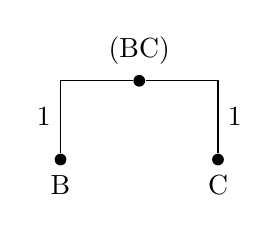
\begin{tikzpicture}
        \path node[punkt, label=above:(BC)] (BC) at (0,0) {}
        node[punkt, label=below:B] (B) at (-1,-1) {} 
        node[punkt, label=below:C] (C) at (1,-1) {};
        \draw   (BC) -| node[near end, left] {1} (B);
        \draw   (BC) -| node[near end, right] {1} (C);
    \end{tikzpicture} 
\end{center}
\paragraph*{\stepfour}
\begin{align*}
    d_{A, (BC)} & = \frac{d_{AB} + d_{AC}}{2}   = \frac{8+8}{2} = 8 \\
    d_{D, (BC)} & = \frac{d_{DB} + d_{DC}}{2}   = \frac{12+12}{2} = 12 \\
    d_{E, (BC)} & = \frac{d_{EB} + d_{EC}}{2}   = \frac{4+4}{2} = 4
\end{align*}
\paragraph*{\stepfive}
\[
\begin{array}{c|ccccc}
  & A & (BC) & D & E \\
\hline
A & 0& 8 & 12& 8 \\
(BC) &  & 0 & 12 & 4 \\
D &  &   & 0 & 12 \\
E &  &   &   & 0
\end{array}
\]
\subsubsection*{Second interation}
\paragraph*{\stepone}
\[d_{(BC),E} = 4\]
\paragraph*{\steptwo}
New cluster: ((BC)E)
\paragraph*{\stepthree}
\[l_{(BC)E} := 4 /2 = 2\] \\
\begin{center}
    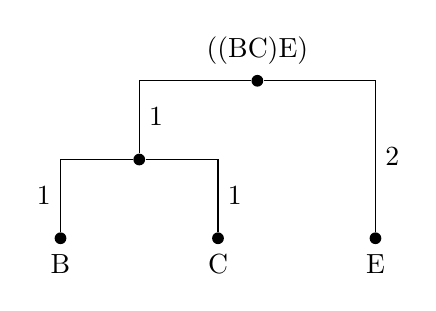
\begin{tikzpicture}
    \path node[punkt] (BC) at (0,0) {}
        node[punkt, label=below:B] (B) at (-1,-1) {}
        node[punkt, label=below:C] (C) at (1,-1) {}
        node[punkt, label=below:E] (E) at (3,-1) {}
        node[punkt, label=above:((BC)E)] (BCE) at (1.5,1) {};
       \draw   (BC) -| node[near end,left] {1} (B);
        \draw   (BC) -| node[near end,right] {1} (C);
        \draw   (BCE) -| node[near end,right] {2} (E);
        \draw   (BCE) -| node[near end,right] {1} (BC);
    \end{tikzpicture}
\end{center}
\paragraph*{\stepfour}
\begin{align*}
    d_{A, ((BC)E)} & = \frac{d_{A(BC)} + d_{AE}}{2}   = \frac{8+ 8}{2} = 8 \\
    d_{D, ((BC)E)} & = \frac{d_{A(BC)} + d_{AE}}{2}   = \frac{12 + 12}{2} = 12
\end{align*}
\paragraph*{\stepfive}
\[
\begin{array}{c|ccccc}
  & A & ((BC)E) & D \\
\hline
A & 0& 8 & 12 \\
((BC)E) &  & 0 & 12  \\
D &  &   & 0
\end{array}
\]
\subsubsection*{Third iteration}
\paragraph*{\stepone}
\[d_{((BC)E),A = 8}\]
\paragraph*{\steptwo}
New cluster: (A((BC)E))
\paragraph*{\stepthree}
\[l_{BC} := 8 /2 = 4\] \\
\begin{center}
    \begin{tikzpicture}
    \path node[punkt] (BC) at (0,0) {}
        node[punkt, label=below:B] (B) at (-1,-1) {}
        node[punkt, label=below:C] (C) at (1,-1) {}
        node[punkt, label=below:E] (E) at (3,-1) {}
         node[punkt, label=below:A] (A) at (5,-1) {}
        node[punkt, label=above:(A((BC)E))] (ABCE) at (3.5,3) {}
        node[punkt] (BCE) at (1.5,1) {};
       \draw   (BC) -| node[near end,left] {1} (B);
        \draw   (BC) -| node[near end,right] {1} (C);
        \draw   (BCE) -| node[near end,right] {2} (E);
        \draw   (BCE) -| node[near end,right] {1} (BC);
        \draw   (ABCE) -| node[near end,right] {2} (BCE);
        \draw   (ABCE) -| node[near end,right] {4} (A);
    \end{tikzpicture}
\end{center}
\paragraph*{\stepfour}
\begin{align*}
    d_{D, (A((BC)E))} & = \frac{d_{((BC)E)} +d_{DA}}{n_{2} }  = \frac{12 + 12}{2} = 12
\end{align*}
\paragraph*{\stepfive}
\[
\begin{array}{c|ccccc}
  &  (A((BC)E)) & D \\
\hline
(A((BC)E)) & 0 & 12  \\
D &    & 0
\end{array}
\]

\subsubsection*{Finale}
Join the last cluster. 
\[ l_{D, (A((BC)E))} = 12 / 2 = 6\]

\newcommand{\wpgma}[0]{ \begin{tikzpicture}
    \path node[punkt] (BC) at (0,0) {}
        node[punkt, label=below:B] (B) at (-1,-1) {}
        node[punkt, label=below:C] (C) at (1,-1) {}
        node[punkt, label=below:E] (E) at (3,-1) {}
         node[punkt, label=below:A] (A) at (5,-1) {}
         node[punkt, label=below:D] (D) at (7,-1) {}
        node[punkt] (ABCE) at (3.5,3) {}
         node[punkt] (ABCDE) at (5.5,5) {}
        node[punkt] (BCE) at (1.5,1) {};
       \draw   (BC) -| node[near end,left] {1} (B);
        \draw   (BC) -| node[near end,right] {1} (C);
        \draw   (BCE) -| node[near end,right] {2} (E);
        \draw   (BCE) -| node[near end,right] {1} (BC);
        \draw   (ABCE) -| node[near end,right] {2} (BCE);
        \draw   (ABCE) -| node[near end,right] {4} (A);
         \draw   (ABCDE) -| node[near end,right] {6} (D);
         \draw   (ABCDE) -| node[near end,right] {2} (ABCE);
    \end{tikzpicture}}
\begin{center}
   \wpgma
\end{center}

\newpage 

\subsection*{Comparison}

\begin{figure}
    \centering
    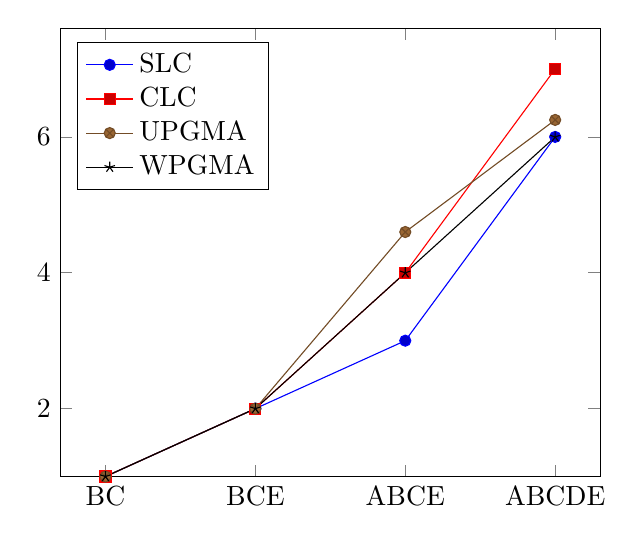
\begin{tikzpicture}
  \begin{axis}[ 
    x tick label style =
      {/pgf/number format/set thousands separator={}},
    legend pos = north west,
    xtick=data,
    ymin=1,
    symbolic x coords={BC,BCE,ABCE,ABCDE},
    legend cell align=left ]
  \addplot coordinates {(BC,1) (BCE,2) (ABCE,3) (ABCDE,6)};
  \addplot coordinates {(BC,1) (BCE,2) (ABCE,4) (ABCDE,7)};
  \addplot coordinates {(BC,1) (BCE,2) (ABCE,4.6) (ABCDE,6.25)};
  \addplot coordinates {(BC,1) (BCE,2) (ABCE,4) (ABCDE,6)};
  \legend{SLC, CLC, UPGMA, WPGMA}
  \end{axis}
\end{tikzpicture}
    \caption{Visualisation of the heights the same nodes get by using different agglomerative clustering methods.}
    \label{fig:my_label}
\end{figure}

\begin{figure}[H]
    \centering
    \begin{subfigure}{0.45\textwidth}
      \resizebox{7cm}{!}{\slcluster}
    \end{subfigure}
    \begin{subfigure}{0.45\textwidth}
      \resizebox{7cm}{!}{\clcluster}
    \end{subfigure}
    \begin{subfigure}{0.45\textwidth}
      \resizebox{7cm}{!}{\upgma}
    \end{subfigure}
    \begin{subfigure}{0.45\textwidth}
      \resizebox{7cm}{!}{\wpgma}
    \end{subfigure}
    \caption{Trees that resulted from using different agglomerative clustering methods on the same distance matrix.}
    \label{fig:my_label}
\end{figure}

\begin{tikzpicture}

\end{tikzpicture}

